\documentclass[11pt, oneside]{article}   	% use "amsart" instead of "article" for AMSLaTeX format
\usepackage{geometry}                		% See geometry.pdf to learn the layout options. There are lots.
\geometry{letterpaper}                   		% ... or a4paper or a5paper or ... 
%\geometry{landscape}                		% Activate for rotated page geometry
%\usepackage[parfill]{parskip}    		% Activate to begin paragraphs with an empty line rather than an indent
\usepackage{graphicx}				% Use pdf, png, jpg, or eps§ with pdflatex; use eps in DVI mode
								% TeX will automatically convert eps --> pdf in pdflatex		
\usepackage{amssymb}
\usepackage{hyperref}

\usepackage{color}
\usepackage{subcaption}
\usepackage{caption}
\usepackage[margin=10pt,font=small,labelfont=bf,
labelsep=endash]{caption}


\newcommand{\todo}[1]{ \textcolor{red}{\bf{To Do:} #1}}
\newcommand{\toref}[1]{ \textcolor{blue}{\bf{REFERENCE #1}}}
\newcommand{\future}[1]{ \textcolor{green}{\bf{Future Direction: #1}}}

%SetFonts

%SetFonts


\title{9 Month TAP Report}
\author{Me :)}
\date{}							% Activate to display a given date or no date

\begin{document}
\maketitle

\section{Low Temperature Plasmas and Wound Healing}
\begin{itemize}
\item Wound statistics. Try to find some up to date stats, possibly UK and globally.
\item Standard wound care protocols and their pros and cons
\item Aim for low temperature plasmas
\item Briefly what has been seen before
\item Brief summary of all the lit review I did for the last TAP on LTP/bio interactions - refs from there :)
\end{itemize}

\subsection{Project Aims}

\begin{enumerate}
\item Development of air plasma - suitable for optical diagnostics \& treatment of biological samples
\item Characterisation of plasma - Experimental \& Computational. Optical diagnostics will be used to determine species densities in the plasma, whilst a global model will be developed alongside to be able to help with species density predictions and guiding of experiments.
\item Biology experiments - Oxidative Stress \& Healing Promotion
\item Correlation between plasmas and biological results - Is there evidence to correlate particular species to particular biological responses?
\end{enumerate}


\section{Work to Date}
\subsection{Simulations}
Previously:
\begin{itemize}
\item GlobalKin - 0D global plasma chemistry model
\item PumpKin - pathways analysis tool
\item Nitrogen chemistry set - as a first step to a air plasma model, nitrogen is a good start. Previously I presented the chemistry set so far. It has 31 species and over 200 reactions involving electrons, heavy particles and some vibrational kinetics.
However, I also pointed out that some areas were missing, in particular some vibrational kinetics.
\end{itemize}

\subsection{Vibration-vibration reactions in nitrogen plasmas}
\begin{itemize}
\item V-V reactions are important to include.... Why?
\item \begin{equation} N_2(X,v=w) + N_2 (X,v=n) \rightarrow N_2(X,v=w-1) + N_2(X,v=n+1)
\label{eqn:V-V} \end{equation}
\item The rates are not widely available, other than for n = 1 $\rightarrow$ 0 and the reverse, n = 0 $\rightarrow$ 1 (\textbf{equation \ref{eqn:V-V}})
\item New paper out by Pintassilgo \cite{Pintassilgo2017modelling} earlier this year shows rates for these VV reactions (n/w = 1 $\rightarrow$ 0 and the reverse, 0 $\rightarrow$ 1), and references equations in \cite{Alves2012capacitively} as the method for calculating the rates.
This would be extremely useful as it would allow calculation of all VV reactions for all values of n/w.
\item However, can't reproduce graph in \cite{Pintassilgo2017modelling}, as shown in \textbf{figure \ref{fig:paper_vs_equations}}.
\item I have since contacted Vasco Guerra and asked him to explain!!
\end{itemize}

\begin{figure}
\includegraphics[width=\textwidth]{Figures/paper_vs_equations}
\caption{VV rates from Pintassilgo and Guerra, 2017 \cite{Pintassilgo2017modelling} shown by the points. VV rates calculated from equations by Alves \textit{et al}, 2012 \cite{Alves2012capacitively} shown by the solid lines. Red shows $N_2(v=1) + N_2(v=w-1) \rightarrow N_2(v=0) + N_2(v=w)$, while the blue represents the reverse reaction}
\label{fig:paper_vs_equations}
\end{figure}

\subsection{Pulsed Plasma Simulations}

\begin{itemize}
\item Experimental nitrogen plasma will be ignited using a pulsed power supply, therefore need to simulate pulsed power too
\item GlobalKin specifies power density in time, therefore, can define power cycle
\item Can show electron kinetics during pulsing, \textbf{figure \ref{fig:pulsed_electrons}}
\end{itemize}

\begin{figure}
\centering
\includegraphics[width=0.6\textwidth]{Figures/pulsed_electrons}
\caption{Figure showing electron densities during pulsed power cycle in GlobalKin}
\label{fig:pulsed_electrons}
\end{figure}

\subsection{Membrane Damage}

\begin{itemize}
\item Aim to look at plasma-induced membrane damage in E.coli MG1655 cells, using the membrane dye FM4-64. Cells prepared by Paulina Dubiel. Picture of setup shown in \textbf{figure \ref{fig:setup_pic}}.
\item The methods
\item Treatment. 

1 mL of cells (OD600 = 2.7) were placed in a well of a 48 well plate, giving a depth of $\approx$ 0.5 cm. 

The plasma jet was positioned so that the tip was 2 cm above the liquid surface. 

Plasma source is a parallel plate configuration. Powered by radio frequency (13.56 MHz), 1 slm He with 5 sccm $O_2$ admixture (0.5 \% $O_2$). Voltage applied was measured using a voltage probe and oscilloscope and was approximately 560 V. \todo{CHECK VOLTAGE. WAS IT 640 V?!}

Treatment times were 30, 60, 90, 120 seconds. Untreated cells were used as a control. Following exposure, cells were stained with FM4-64 dye at \todo{Dilution} then put on microscope slides, covered with coverslip, then sealed with nail varnish.

\item Preliminary results show something or other. As yet I have no idea. Possibly interesting... \textbf{figure \ref{fig:results}}

\item Temperature measured with a thermocouple. For treatments, temperature at approx. 2 cm from plasma tip was $\approx$ X$^\circ$C \todo{temperatures}.
A power variation for the temperature of the plasma effluent was also carried out and the results are shown in \todo{power variation and temperature experiment and graph}
\end{itemize}

\begin{figure}
\centering
\includegraphics[width=0.6\textwidth, angle=270]{Figures/setup_pic}
\caption{Photograph showing the plasma jet and plate containing bacterial}
\label{fig:setup_pic}
\end{figure}

\begin{figure}
\centering
\includegraphics[width=0.5\textwidth]{Figures/cells}
\caption{Picture showing the 120 s treated E.coli. Red is membrane, yellow is everything and black is non-fluorescing stuff...}
\label{fig:results}
\end{figure}


\section{Future Directions}

\subsection{Simulations}

\begin{itemize}
\item Add in appropriate V-V and V-T reactions and rates
\item Check about pressures - anything missing due to difference between low and atmospheric pressure?
\item Start adding in oxygen species/reactions following benchmarking of model, or simultaneously using proper version control!!
\end{itemize}

\subsubsection{Benchmarking of Nitrogen Model}

\begin{itemize}
\item Need a plasma source for pure nitrogen plasma to benchmark model
\item Parallel plate configuration. Nanosecond pulses. Anything else electric-y?
\item Picture of source? \todo{Take a picture of source!} \textbf{figure \ref{fig:plasma_source}}
\item Take measurements of atomic nitrogen
\item TALIF?
\end{itemize}

\begin{figure}
\centering
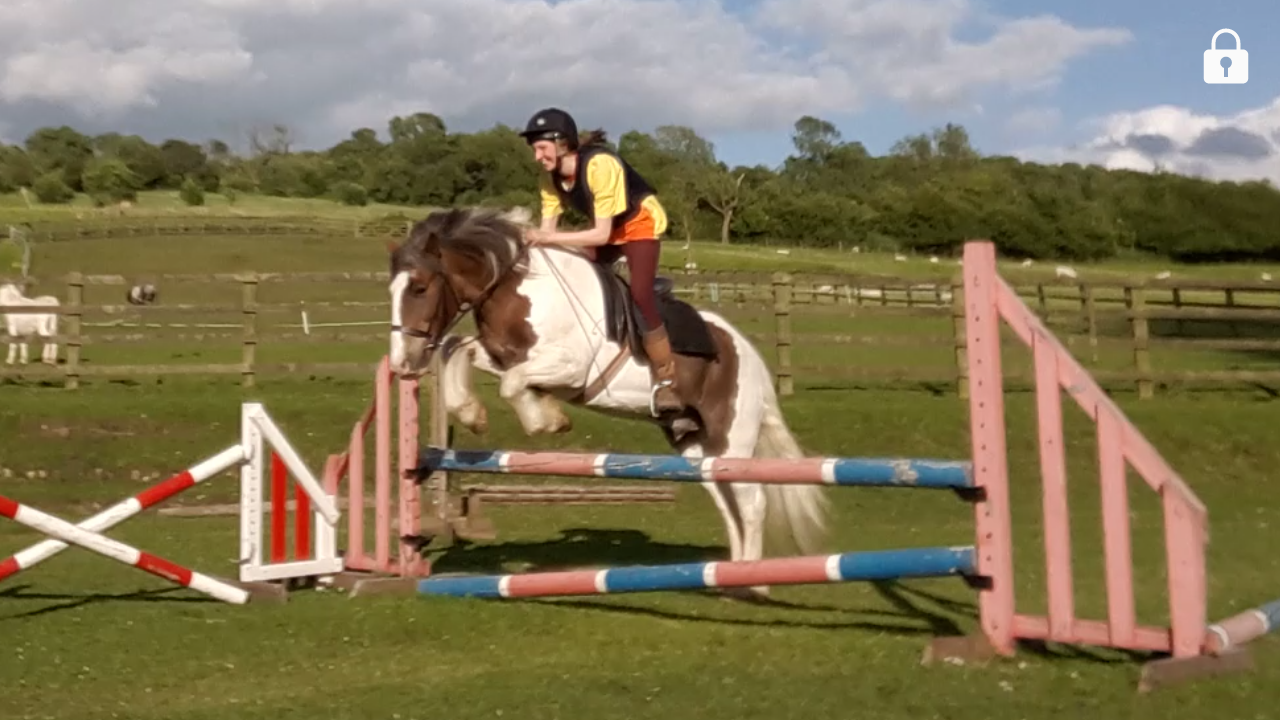
\includegraphics[width=\textwidth]{Figures/Harry}
\caption{Haribo}
\label{fig:plasma_source}
\end{figure}

\subsection{Biology Aims}

\begin{itemize}
\item Wound healing is of interest. For the time being, host cells will be investigated. Particularly important from a safety point of view, as well as the potential for promoting the healing response
\item Need to decide on the experiment end point, i.e. what to measure
\item Oxidative Stress?
\item Wound Healing?
\end{itemize}

\subsubsection{Human Skin}

The skin has different layers. The following information about skin layers comes from: 

\url{https://opentextbc.ca/anatomyandphysiology/chapter/5-1-layers-of-the-skin/}


There is the epidermis, the dermis and the hypodermis.
The epidermis it the most superficial layer, exposed to the environment, and is composed almost entirely of keratin-producing cells, keratinocytes.
The epidermis is made up of different layers, namely from deep to superficial, the stratum basale, stratum spinosum, stratum granulosum and stratum corneum.
All except the stratum basale is made of keratinocytes, whereas the stratum basale consists mainly of basal cells (which are keratinocyte precurosrs), but also contains Merkel cells (touch receptors) and melanocytes (melanin-producing cells).
As basal cells divide and produce daughter keratinocytes, the keratinocytes are pushed up through the epidermal layers, producing increasing amounts of keratin and then dying, leaving begin the keratin and cell membranes, so that the most superficial layer consists only of dead keratinocytes and their keratin.
The epidermis also contains Langerhan's cells, which are a skin-specific dendritic cell, which is able to phagocytose invading pathogens and debris.

The dermis is below the epidermis and contains structures such as blood vessels, hair follicles and sweat glands, in dense, irregular connective tissue.
Finally, the hypodermis consists mainly of loose connective tissue and fatty tissue.

A real paper on skin structure \cite{Mancini2014microRNAs}...

When considering wound treatments using LTP, depending on the type and severity of the wound, the skin cells that will be exposed will vary.
However, since keratinocytes form the bulk of the epidermis, it is reasonable to start any investigations of LTP effects on skin cells in these cells.



\subsubsection{Plasma-Induced Oxidative Stress in Human Skin Cells}

Oxidative stress is when cells/tissues are overwhelmed by oxidants. 
Oxidants are things which cause oxidation.
Free radical chain reactions normally produce numerous non-radical oxidants, such as hydrogen peroxide \todo{reference: https://hstalks.com/t/374/introduction-to-free-radicals-and-the-oxygen-parad/?biosci} .

Oxidative stress can lead to induction of lipid peroxidation and modulation in the levels of antioxidant and drug-metabolising enzymes.
ROS have also been demonstrated to induce some transcription factors, such as activating protein 1 (AP-1), and NF-$\kappa$B. 
UVA is also involved in NF-$\kappa$B activation.
Mitogen-activated protein kinase (MAPK) pathway is also a target of oxidative stress \cite{Bickers2006oxidative}.

\cite{Nadal2011controlling} - paper talking about different sensors/transduction mechanisms/effectors but mainly in yeast and drosophilia

\cite{Bickers2006oxidative} - another paper talking specifically about the skin and the role of oxidative stress in disease

Kim2005role - something to do with MAPK in mouse skin following heat treatment

Escuin-Ordinas2016cutaneous - something to do with MAPK, ERK and wound healing!

\paragraph{Oxidative Stress Detection}

\begin{itemize}
\item Cell death
\item Cell membrane integrity, lipid peroxidation products (MDA and 4-HNE), DNA damage. Fluorescent probes could be used \cite{Ayala2014lipid, Joshi2011nonthermal, Joshi2010control}
\item RNA???
miRNA in wound healing \cite{Riemondy2014not} - a review suggests wound healing promoted by miR-99 downregulation, and others may also be involved in wound healing. Downregulation of miR-199a-5p and miR-200b supports angiogenesis.

miR-200c is involved in wound healing. Downregulation is required for proper healing as upregulation inhibits cell migration during wound repair  \cite{Aunin2017exploring}. 
miR-200c is also upregulated by oxidative stress \cite{Magenta2011miR}. Yay.

miR-25??
\end{itemize}

\subsubsection{Oxidative Stress Experiments}
method for looking at RNA expression

\future{Speak to Dmitris/read etc}

\subsection{Biology Aims - Wound Healing Promotion}

Scratch test, MatTek skin, Gene expression

Do keratinocytes need to be wounded to be able to induce the wound healing promotion?! Or is the role of oxidative stress different in wounded and healthy keratinocytes??

\subsection{COST jets}

COST jets are reference microplasma sources, designed to all be the same so that plasmas can be produced consistently by the different sources.
The four jets have all been investigated in terms of \todo{Find out what Fred has done}, and the aim is to carry out a simple bacterial killing assay, to determine the killing zone of each of the four jets so they can be compared. 

Power, temperature, emission

To do this, \textit{E. coli} MG1655 will be used. 
Bacteria will be grown, then plated onto agar plates, before being exposed to the plasma jet. 
The plates will then be incubated, and colonies counted and pictures taken, to determine the extent of the area of bacteria that has been killed by the plasma.

\subsubsection{Methods}
Blah blah blah.... This is how you grow bacteria.....

\section{Immediate Plans}
In the immediate future, an experiment for monitoring oxidative stress in skin cells needs to be developed. 
To do this, as well as the information from the literature review, I am also meeting with Dmitris Lagos, an RNA expert, to discuss the role of RNA in the stress response...


\section{Project Outlook}
















%\section{Oxidative Stress}
%Oxygen derived species - $\cdot$OH, O$_2^-\cdot$ and H$_2$O$_2$. However, O$_2^-\cdot$ and H$_2$O$_2$ have a low chemical reactivity, and do not readily react with biological molecules such as DNA, proteins and lipids. On the other hand, $\cdot$OH is very highly reactive, with reaction rates at or near diffusion-controlled rates for reactions with DNA \cite{Dizdaroglu2012oxidatively}.
%
%\subsection{DNA Damage}
%
%
%\section{Detecting Oxidative Stress - Bacteria}
%Different ways of detecting oxidative stress in bactera.
%In general, things to look for are cell death, membrane damage, DNA damage, lipid peroxidation and functional changes in proteins (e.g. enzyme deactivation).
%
%\subsection{Cell death}
%Measuring cell death can be done by measuring population level cell death, e.g through looking at zones of inhibition etc or at cellular level, e.g. using exclusion dyes.
%
%\subsection{Lipid Peroxidation}
%\begin{itemize}
%\item Lipid - large molecules made from smaller units of fatty acids and glycerol 
%\item Fatty acid - carboxylic acid consisting of a hydrocarbon chain and a terminal carboxyl group.
%\end{itemize}
%
%Radicals can attack polyunsaturated fatty acids and initiate lipid peroxidation in membranes.
%This can have significant effects on membrane fluidity and membrane-bound proteins.
%As a result of lipid peroxidation, aldehydes are often formed, which are long lived and able to function as "toxic second messenger" molecules, which can cause further damage to cells, in particular proteins \cite{Cabiscol2000oxidative}.
%These products include malonaldehyde (MDA) and 4-hydroxynonenal (HNE), which are particularly mutagenic and toxic, respectively \cite{Ayala2014lipid}.
%
%\subsection{DNA damage}
%
%\section{Methods}
%
%\begin{itemize}
%\item XTT assay. Metabolic activity
%
%Paper talking about oxidative stress in bacteria \cite{Cabiscol2000oxidative}. Talks about attack on lipids, proteins and DNA.
%
%\cite{Ezraty2017oxidative} is a paper with lots of biochemistry-y stuff in. Haven't read it - think it is a bit too in depth all about the mechanisms of protein damage, in particular sulphur containing side chains of proteins.
%
%\cite{Alkawareek2014potential} Paper looked at LTP interactions with bacteria, in particular bacterial killing/metabolism XTT assay (E. Coli, P. aeruginosa, B. cereus and MRSA), plasmid DNA damage (single and double strand breaks by looking whether the plasma was supercoiled (undamaged), open circular (single strand break) or linear (double strand break)), protein function (proteinase K's function was watched to see if the plasma was altering the structure in some way to prevent catalytic activity (it is pretty robust to changes in temp and pH therefore decrease in activity likely to be due to structural changes)), lipid peroxidation (MDA measurement in E. Coli) and membrane permeability (by measuring ATP leakage from E. Coli).
%\end{itemize}
%
%Assays:
%\begin{enumerate}
%\item \url{https://www.caymanchem.com/product/589320} - DNA/RNA Oxidative Damage ELISA Kit. Looks for 8-hydroxy-2'-deoxyguanosine from DNA, 8-hydroxyguanosine from RNA, and 8-hydroxyguanine from either DNA or RNA.
%\item
%\end{enumerate}
%%\section{}
%%\subsection{}
%
%\section{Detecting Oxidative Stress - Skin Cells}
%
%
%
%\section{Skin Models for Wound Healing Assays}
%Skin explants (people) can be cultured (as an organ culture) for up to 2 weeks at the air/liquid interface \cite{Gottrup2000models}.
%\subsection{Porcine Skin}
%
%\subsection{Hyaluronic Acid}
%
%\section{Cancer Things}
%\subsection{Radiotherapy}
%Radiation therapy can either be photon or particle, radiation.
%Photon radiation uses gamma ray or x ray beams focussed on the tumour, whereas particle radiation uses electrons, neutrons or protons for the same purpose - energy deposition into the tumour.
%By targeting the tumour with these beams, they deposit energy in the tumour cells, and cause ionisation of particles in the cells.
%This then leads to radical formation etc which causes damage to cancer cell DNA and prohibits their replication.
%Healthy cells are generally better at repairing DNA defects, meaning that if doses are delivered that cause sub-lethal levels of damage to healthy cells, then the healthy cells have time to repair before the next dose (as they divide much more slowly than cancer cells, so have longer to repair damage), whereas, cancer cells don't and therefore die.
%This gives specificity of a fashion.
%Damage to DNA occurs both directly (ie, the radiation directly damages the DNA), or indirectly, through formation of radical species which then attack the DNA. \cite{Baskar2012cancer}
%
%
%\subsection{Immunotherapy}
%\subsection{Photodynamic therapy}



\scriptsize
\bibliographystyle{ieeetr}
\bibliography{/Users/hld523/Bibliography/MyPapers}
\end{document}  